\documentclass{article} % For LaTeX2e
\usepackage{nips13submit_e,times}
\usepackage{hyperref}
\usepackage{url}
\usepackage{tikz}
\usetikzlibrary{arrows}
\usepackage{graphicx}
\usepackage{csquotes}
\usepackage{placeins}
\usepackage{booktabs} % To thicken table lines
%\documentstyle[nips13submit_09,times,art10]{article} % For LaTeX 2.09


\title{Understanding pro-social landing: How lenders respond to loan descriptions on Kiva
}


\author{
Zi Yin \\
Department of Electrical Engineering\\
Stanford University\\
\texttt{zyin@stanford.edu} \\
\And
Yuanyuan Shen \\
Graduate School of Business \\
Stanford University \\
\texttt{yyshen@stanford.edu} \\
}

% The \author macro works with any number of authors. There are two commands
% used to separate the names and addresses of multiple authors: \And and \AND.
%
% Using \And between authors leaves it to \LaTeX{} to determine where to break
% the lines. Using \AND forces a linebreak at that point. So, if \LaTeX{}
% puts 3 of 4 authors names on the first line, and the last on the second
% line, try using \AND instead of \And before the third author name.

\newcommand{\fix}{\marginpar{FIX}}
\newcommand{\new}{\marginpar{NEW}}

%\nipsfinalcopy % Uncomment for camera-ready version

\begin{document}


\maketitle

\section{Introduction}
Kiva is one of the world's first online philanthropic microcredit crowdsourcing platform. Its mission is to connect people through lending to alleviate poverty. Founded in 2005, Kiva has attracted more than 2 million lenders and raised more than 700 million dollars with a 98.6\% repayment rate. 

On the demand side, Kiva partnered with local microcredit lending agencies in the third world to screen the borrowers and post their requests online. On the supply side, Kiva connects lenders online to fund the loans in increments of \$25 dollars. The lenders are philanthropists who do not charge any interest for the loan. They browse through Kiva's online platform and select a fundraising loan to contribute. Each loan is listed on the website for up to a month (with some exceptions). Loans that are not fulfilled within a month will be expired.  Depending on its amount, purpose (e.g. for education, for business) and description, each loan is funded at a different speed. 

To remain competitive in the market, Kiva wants its loans to be funded as fast as possible. In this project, we will study how the loan descriptions will affect the funding speed of the loans. This is crucial for Kiva to provide guidance to its partners who write the descriptions for the loans. 

In particular, we will investigate how loan descriptions affect the loan fulfillment days, and provide suggestions on how to write a good loan description to have one's loan quickly fulfilled.



\section{Problem statement}
We obtained Kiva's loan data from its API website. A data snapshot as of Dec 18, 2015 contains the information cumulative through that date. Table \ref{features} summarizes the features of the loans we are able to obtain from the data set. We know whether each loan was fully funded and how fast it was funded. The funding time, ranging from 0 to 80 days, is the output for our model. The loan descriptions are paragraphs ranging from 50 to 300 words in length. We will apply models of deep learning in NLP to predict the funding speed and see which words and phrases are linked to higher fulfilling rate.  We will also use the features in Table \ref{features} as inputs to the hidden layers. A relevant study by Liu et al.\ [1] evaluates the impact of lenders' motivations on their funding enthusiasm applying standard Natural Language Processing models. They found that certain phrases in the lenders' motivations (filled online upon registration) are associated with higher activity levels. Here we will study the online platform from a demand side.  Our work is also related to word classification of user-generated content and social media e.g., [2, 3]). 

\begin{table}[ht]
\centering
\caption{Features for each loan}
\label{features}
\begin{tabular}{llr}
\multicolumn{1}{c}{\bf Variable}  &\multicolumn{1}{c}{\bf Description}   &\multicolumn{1}{c}{\bf Type}\\ \hline
Status  &  Status of the loan (funded, repaid, etc) & Categorical       \\
Sector  & Purpose of the loan defined by Kiva     &  Categorical\\
Loan description & Story that explains the purpose of the loan & String \\
Loan amount & Amount that the borrower(s) requests  & Numerical      \\
Funded amount & Amount that has been raised on Kiva   & Numerical     \\
Delinquent & Whether the repayment was delayed & Binary 
\\
Partner ID & Id of the partner that manages the loan & Categorical
\\
Posted date & Date that the loan was posted on Kiva  & Time     \\
Funded date  & Date that the loan was fully funded on Kiva  & Time     \\
Planned expiration date & Planned date of fundraising expiration  & Time     \\
Disbursal date & Date that the loan is actually disbursed to the borrower(s) & Time \\
Borrower(s)'s gender & The gender of the borrower(s) & List of Binary \\ \bottomrule
\end{tabular}    
\end{table}
\FloatBarrier

Our goal is to incorporate the loan descriptions as an important predictor of the loan fulfillment speed. Each description is a paragraph with an example given below:

\begin{displayquote}
Tuipulotu T., 19, is single with no children.  She has many years of experience in the Elei (traditional fabric printing) business. She sells to the general public 6 days per week. She has 2 previous loans with SPBD.  She expects her weekly net cash flow to be 600 Tala (\~250 USD).  SPBD loans are Tuipulotu 2019s only access to capital because she was never able to qualify for a loan with the traditional banks.
\end{displayquote}
 

We use the square loss, i.e. $||\hat y-y||^2$ where $y$ is the actual fulfilled days. There are several experiments we will run and compare:
\begin{enumerate}
\item The mean square error using the benchmark regression model and features excluding the loan description;
\item The mean square error using only the loan description and the language model;
\item The mean square error when both the loan description and other features are used.
\end{enumerate}

\section{Technical Approach and Models}
TWe first tokenize the loan descriptions. We will apply several different networks (RNNs, LSTMs and Recursive neural networks) and evaluate their performance in terms of mean square errors. 

The Kiva dataset is of size 5.5GB on disk, in its raw form. Since some loan descriptions are written in languages other than English (and hence do not fit in our word embeddings), and some loans have missing entries, we performed a data cleaning procedure before feeding the data into the models. There are 860,000 loans in total after data cleaning.

To train the model, we feed the loan descriptions into the recurrent neural network. At each unfolded time point, the output $\hat y_i^{(t)}$ is the predictor of the loan fulfillment days, and is compared to the true fulfillment day $y_i$. Hence the loss function corresponding to the $i$th data point, with loan description length $T_i$, is
\[\sum_{t=1}^{T_i}(\hat y_i^{(t)}-y_i)^2\]
We then sum over the training set and get the loss function we try to minimize:
\[\textbf{Loss}=\sum_i\sum_{t=1}^{T_i}(\hat y_i^{(t)}-y_i)^2\]


\begin{figure}[ht]
\centering
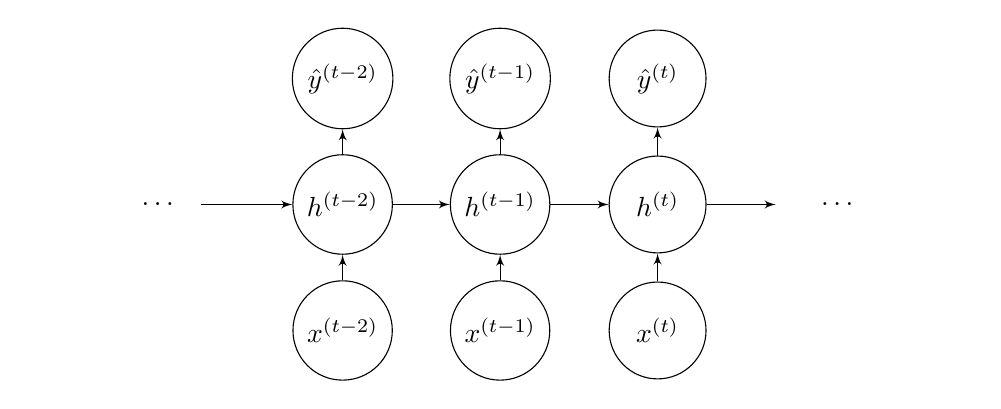
\begin{tikzpicture}

\tikzset{vertex/.style = {shape=circle,draw,minimum size=3.5em}}
\tikzset{edge/.style = {->,> = latex'}}
% vertices
\node[vertex] (a) at  (0,0) {$h^{(t-2)}$};
\node[vertex] (b) at (2,0) {$h^{(t-1)}$};
\node[vertex] (c) at (4,0) {$h^{(t)}$};



\node[vertex] (a1) at  (0,1.6) {$\hat y^{(t-2)}$};
\node[vertex] (b1) at (2,1.6) {$\hat y^{(t-1)}$};
\node[vertex] (c1) at (4,1.6) {$\hat y^{(t)}$};


\node[vertex] (a2) at  (0,-1.6) {$x^{(t-2)}$};
\node[vertex] (b2) at (2,-1.6) {$x^{(t-1)}$};
\node[vertex] (c2) at (4,-1.6) {$x^{(t)}$};

%edges
\draw[edge] (a) to (a1);
\draw[edge] (a2) to (a);
\draw[edge] (b) to (b1);
\draw[edge] (b2) to (b);
\draw[edge] (c) to (c1);
\draw[edge] (c2) to (c);


\draw[edge] (a) to (b);
\draw[edge] (b) to (c);

\draw[edge] (c) to (5.5,0);
\draw[edge] (-1.8,0) to (a);
\path (c) to node {\dots} (8,0);
\path (-4,0) to node {\dots} (a);

\end{tikzpicture}
\caption{Network structure}
\end{figure}

In the end, we will try incorporating the other features in Table \ref{features} to the final hidden layer. 

\newpage
\section{Intermediate/Preliminary Experiments \& Results}
As a benchmark, we regress the funding time for the funded loans on sector, loan amount and partner Id. We get a RMSE of 8.25.

\begin{figure}[ht]
\centering
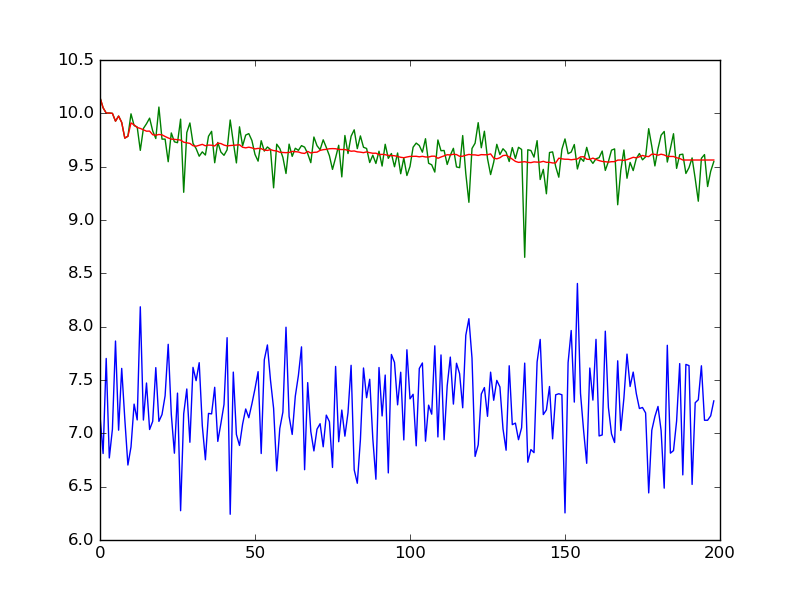
\includegraphics[width=0.75\textwidth]{figure_1.png}
\caption{vanilla RNN training and validation error}
\end{figure}
We implemented a vanilla recurrent neural network, with one hidden layer of 144 neurons. Above is a figure of the training and validation errors during the training process. The blue curve is the training error; the green one represents the validation error (on a test data set), while the red line indicates the moving average. We are able to achieve a RMSE of 6.46 using this network on the final test dataset.


\section*{References}

\small{
[1] Liu et al. (2012) "I Loan Because...": Understanding Motivations for Pro-Social Lending.  {\it WSDM'12}.

[2] Agichtein et al. (2008) Finding high-quality content in social media. In {\it Proceedings of the
international conference on Web search and web data mining}, pages
183-194. ACM, 2008.

[3] Sriram et al. (2010) Short text classification in twitter to improve
information filtering. In {\it Proceeding of the 33rd international ACM
SIGIR conference on research and development in information
retrieval}, pages 841-842. ACM, 2010.

\end{document}
